\documentclass[10pt,twoside]{article} 
\usepackage[a4paper,portrait, top=20mm,bottom=15mm,left=25mm,right=25mm]{geometry}
\author{ }

\usepackage[utf8]{inputenc} 

\usepackage[portuguese]{babel}
\usepackage[T1]{fontenc}

\usepackage{hyphenat} 

\usepackage[dvipsnames]{xcolor}

% Disable all paragraph indentation
\setlength{\parindent}{0pt}

\usepackage{siunitx}
\sisetup{detect-all}

\usepackage{graphicx}
\usepackage{enumitem}

\makeatletter
\renewcommand{\maketitle}{\bgroup\setlength{\parindent}{0pt}
	\begin{center}
		\textbf{\@title}
		
		\@author
	\end{center}\egroup
}
\makeatother


\title{{\Large\bf\center PSD - Projeto Final} 
\\ Implementação de um Banco de Filtros FIR}

%\author{{\bf Autor Um, Autor Dois}}

\date{}


\begin{document}

\maketitle

\vspace{10pt}
\noindent
\begin{tabular*}{\textwidth}{@{\extracolsep{\fill}}@{}l r@{}} %to \textwidth {@{}X[l] X[-1, r]@{}}
	{\bf PSD 2022/2023} & {\bf Turma:} 1MEEC T02\\
	  &  {\bf Jorge Pais e Pedro Duarte} 
\end{tabular*}

\noindent{\rule{\linewidth}{1.5pt}}

%\vspace{20pt}

\section{Introdução}	
O presente relatório tem como finalidade apresentar as atividades desenvolvidas e os resultados obtidos ao longo do projeto final realizado no âmbito da unidade curricular Projeto de Sistemas Digitais.

O principal objetivo deste trabalho passava por conceber um circuito digital para implementar um banco de oito filtros digitais de resposta finita (FIR) diferentes para processamento de um sinal ultrassónico. A saída do circuito é calculada através da convolução discreta entre o sinal de entrada e a resposta impulsional do filtro.

\section{Diagrama de blocos}
De forma a realizar a operação pretendida, o seguinte esquema lógico foi inicialmente projetado para a componente do caminho de dados, representado na Figura 2.1.

\begin{center}
	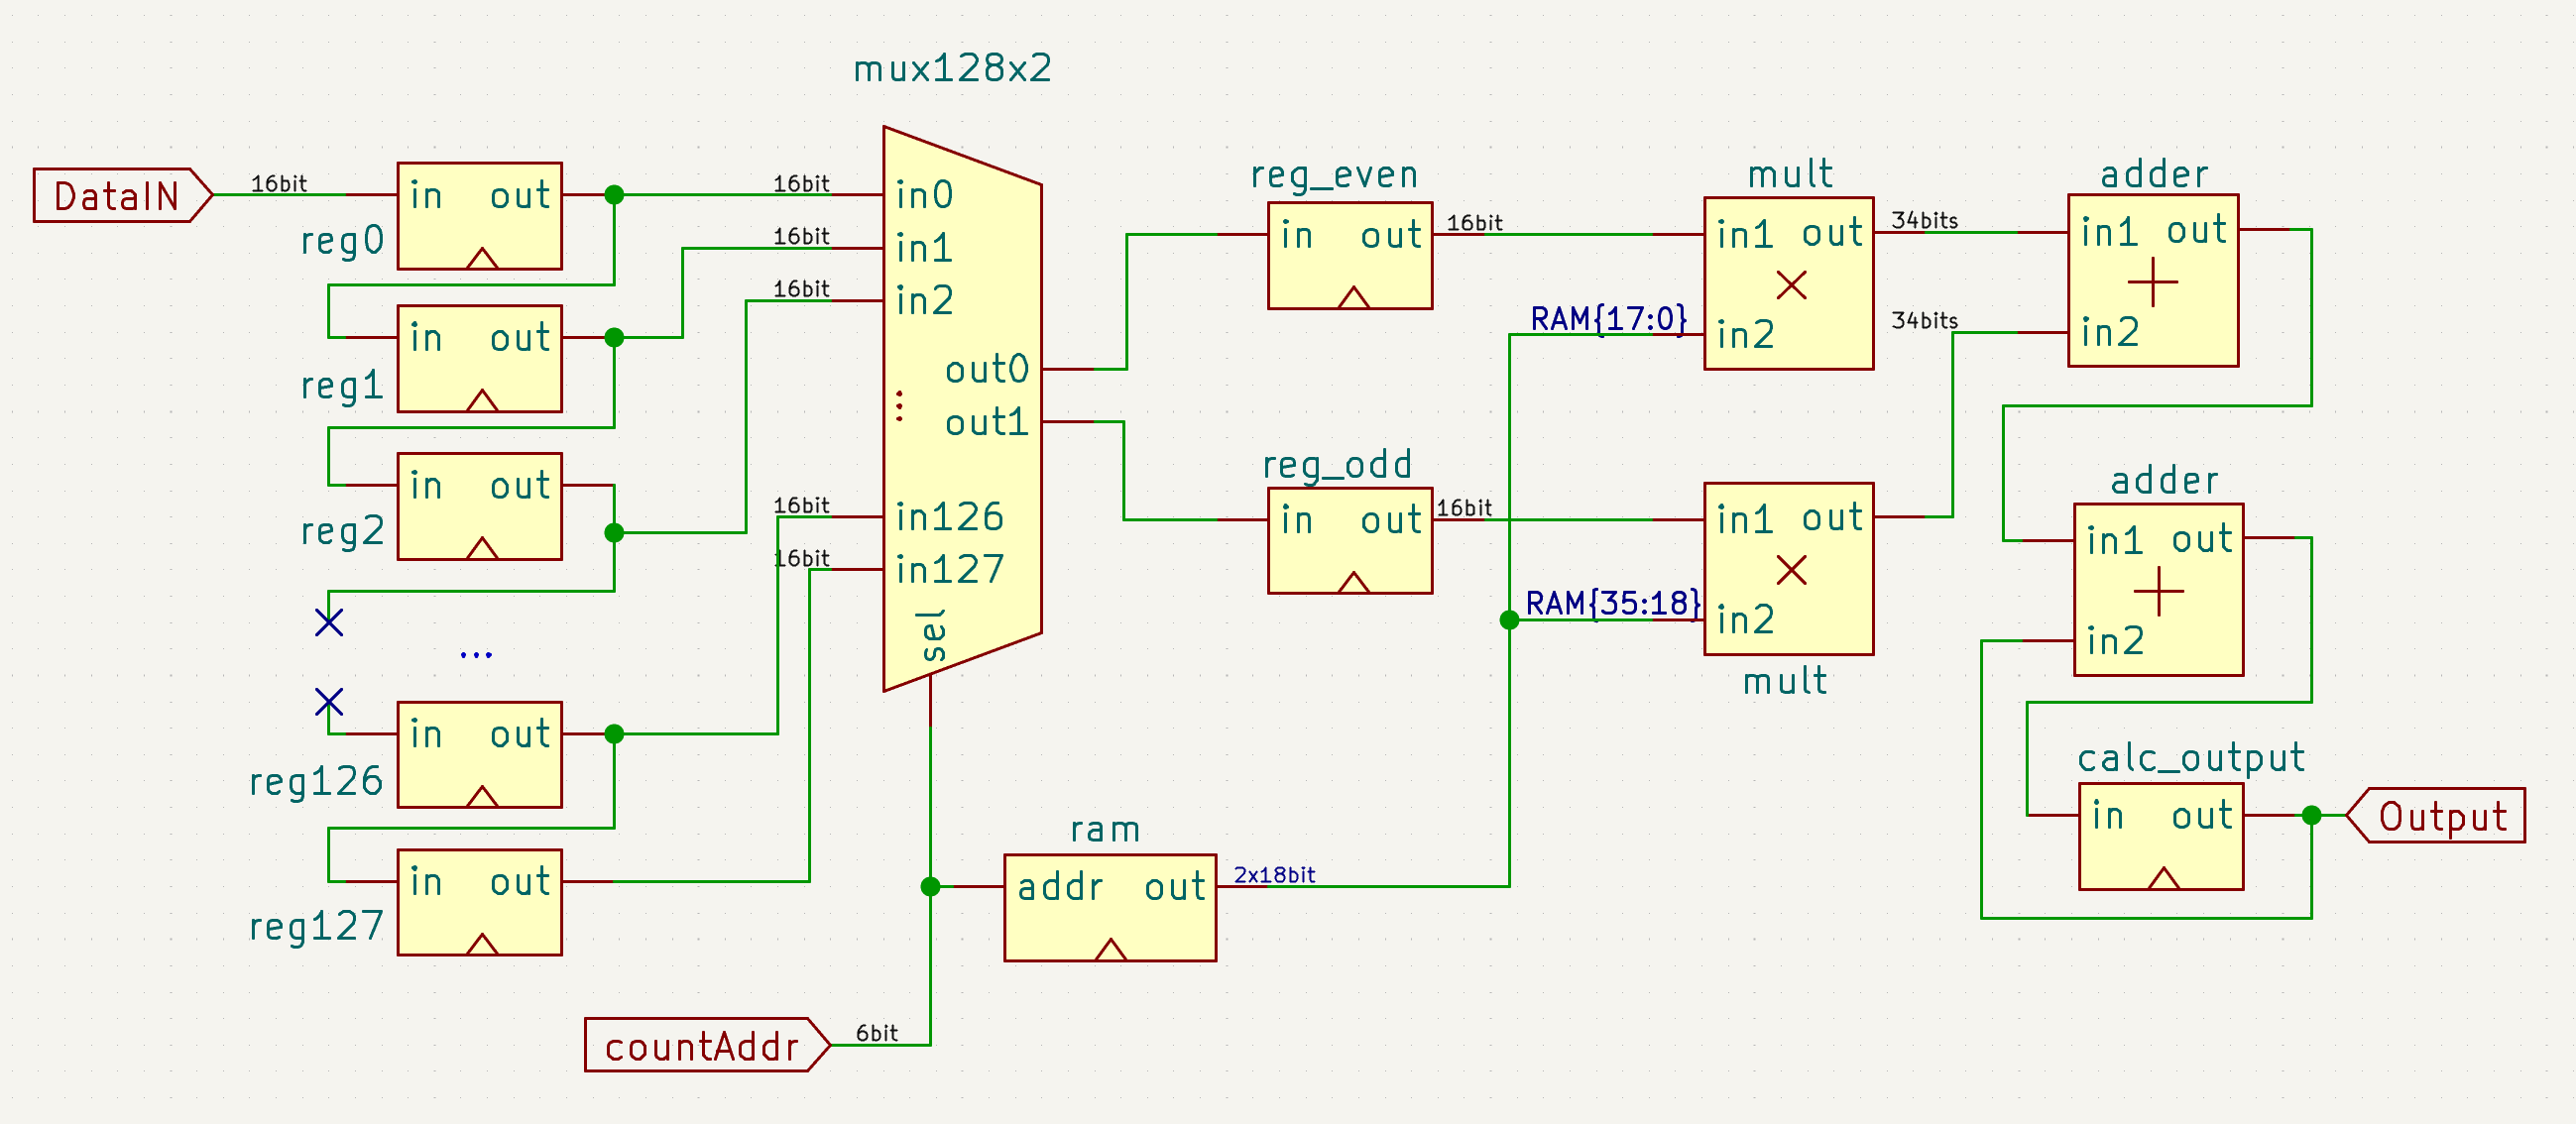
\includegraphics[height=6cm]{figures/simple.png}\\
	Figura 2.1 - Caminho de dados do filtro FIR
\end{center}

O circuito conta com um buffer de 128 registos na entrada, sendo que quando o sinal de \textit{din\_enable} é recebido, o conteúdo de todos os registos é deslocado para o próximo e a nova amostra a receber é armazenada no primeiro registo do buffer. Dado que a memória RAM disponibilizada para o projeto permite ler 2 coeficientes de 18 bits de cada vez, recorreu-se a um multiplexador de 128 para 2, de forma a selecionar cada par de amostras.\
De forma a sincronizar as amostras selecionadas com os coeficientes lidos (dado que a RAM demora 2 ciclos de relógio a retornar o conteúdo do endereço pretendido), dois registos são utilizados depois do multiplexador para atrasar as amostras lidas do buffer. Estes registos também servem de forma a implementar uma arquitetura de pipeline. Com as amostras e os coeficientes prontos para realizar as operações necessárias para os cálculos da saída de cada filtro, estes são multiplicados entre si e o resultado da operação é somado aos conteúdos do registo de saída.

\subsection{Otimizações do Caminho de Dados}
Com o intuito de melhorar a performance do circuito, aumentando o clock e permitindo, assim, que o circuito seja capaz de realizar as operações de filtragem para a maior largura de banda possível, foi implementado pipelining nas operações aritméticas do circuito, separando as multiplicações do processo de acumulação da saída. O esquema lógico do caminho de dados após esta modificação está representado na Figura 2.2, juntamente com a adição de um registo para o qual a saída é carregada após os cálculos terminarem.

\begin{center}
	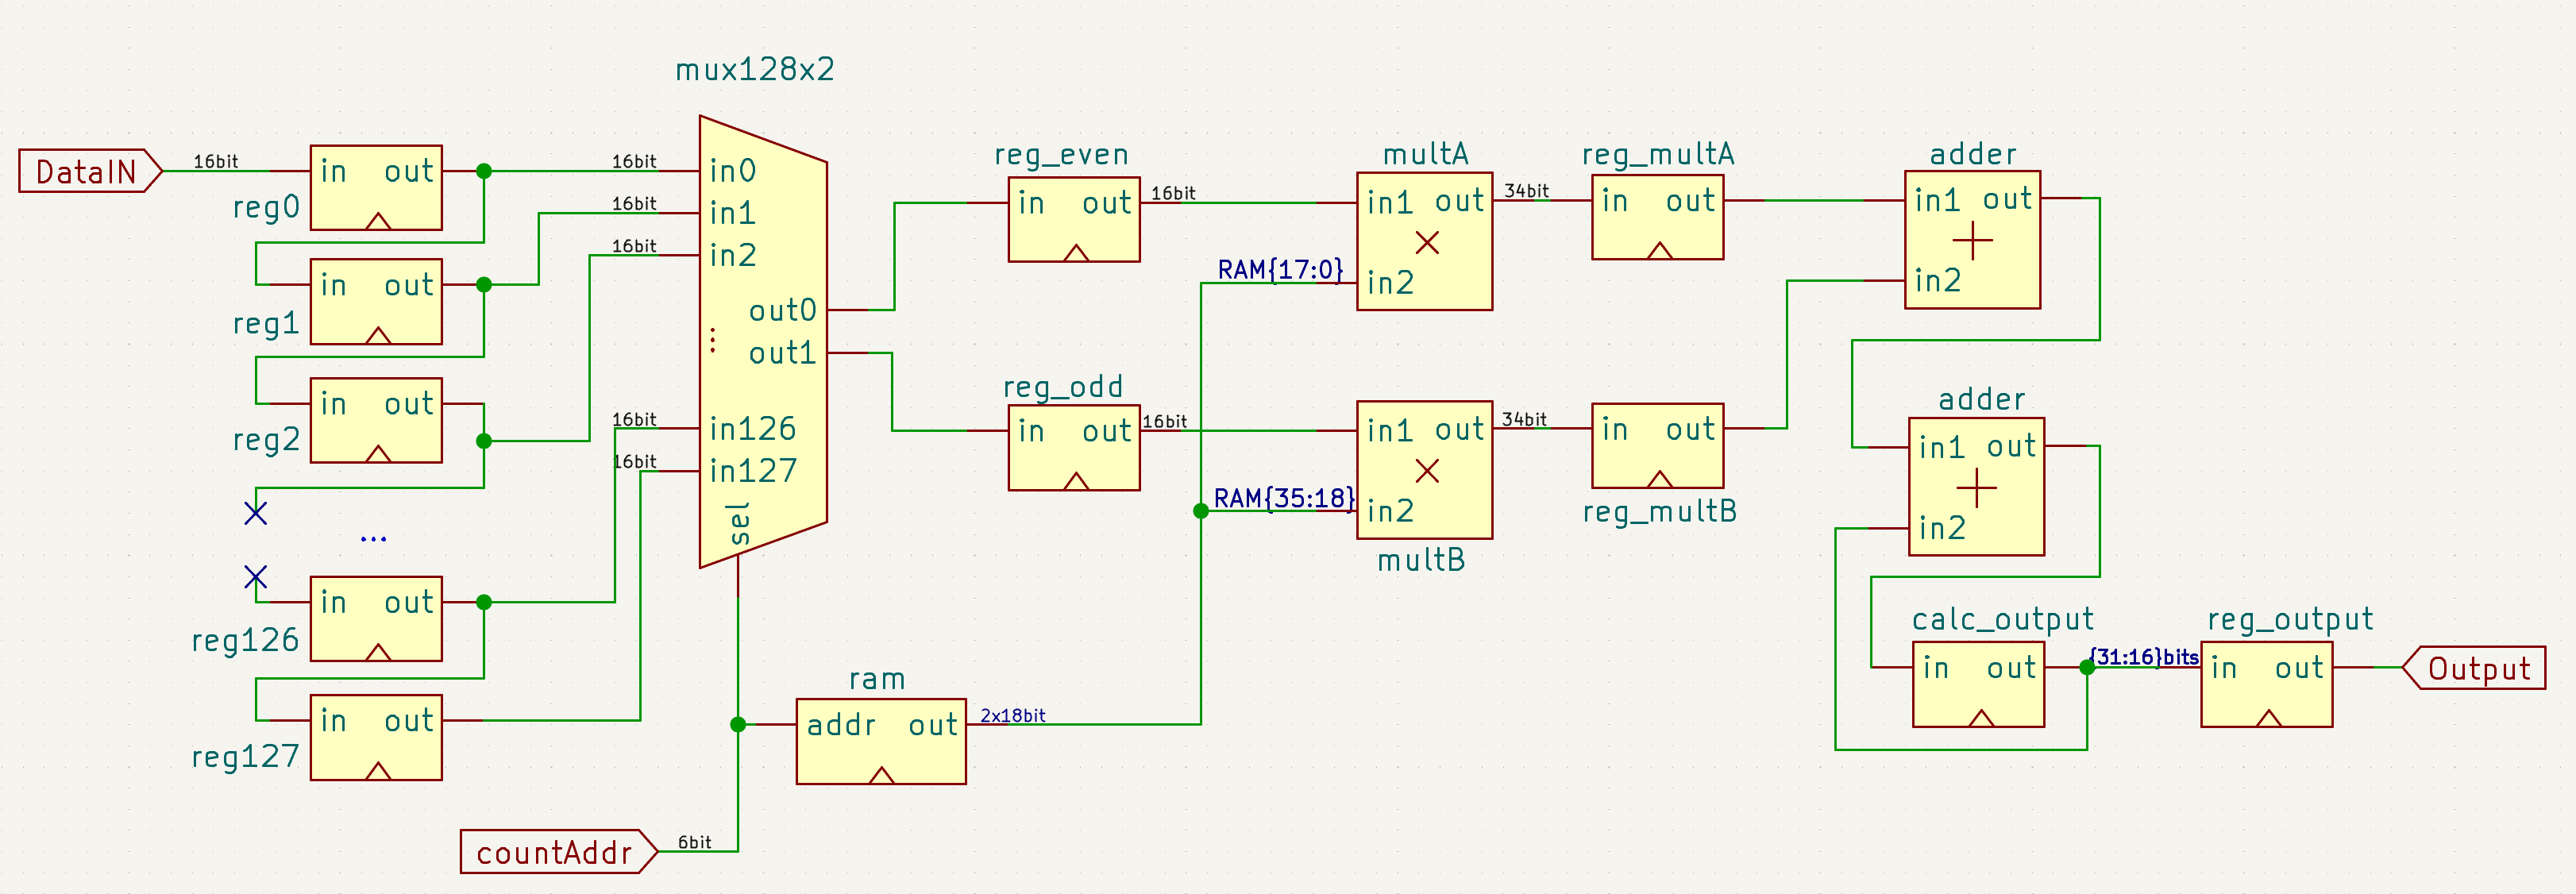
\includegraphics[height=5.5cm]{figures/complete.png}\\
	Figura 2.2 - Caminho de dados do filtro FIR, incluindo \textit{pipelining}
\end{center}

\subsection{Máquina de estados}
Posto isto, concebeu-se uma máquina de estados para controlar o fluxo de dados, a qual está representada de forma sucinta na figura 2.3. O estado INIT funciona, neste caso, como um reset, limpando os dois buffers de saída, o buffer de entrada e os registos de amostra intermédios. No START, é definido o primeiro endereço a ser carregado para as memórias RAM, as saídas são colocadas a zero e o buffer de entrada é carregado com a nova amostra, dando shift em todas as posições. No SET1, apenas se prepara o segundo endereço a ser lido pelas memórias RAM. De seguida, no SET2, os primeiros valores são já multiplicados, além de se preparar o terceiro endereço para ser lido. No estado RUN, o circuito irá calcular, em loop, o output até todos os 64 endereços serem lidos pela RAM.

\begin{center}
	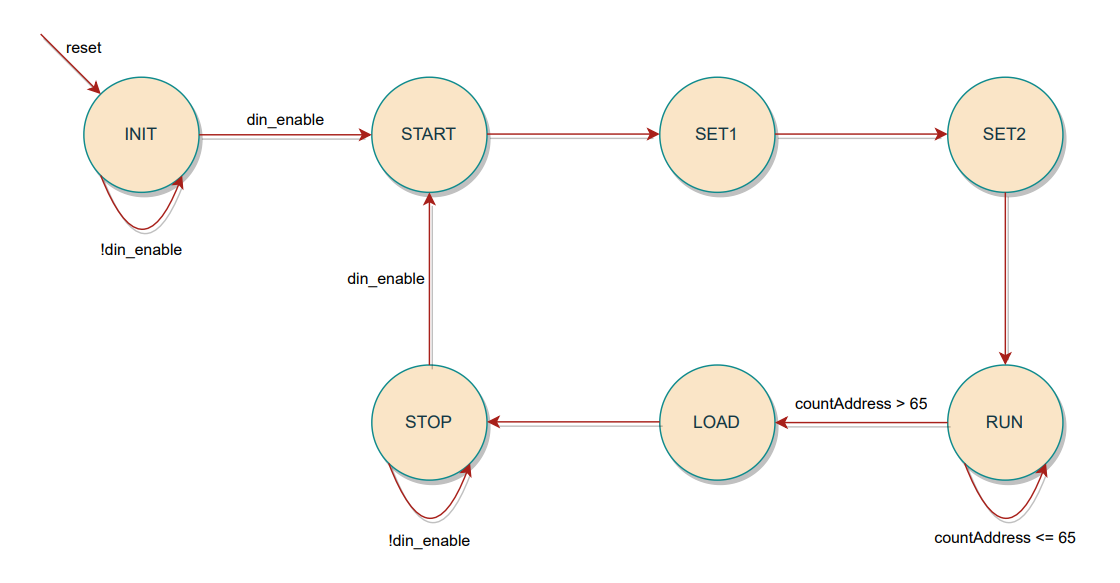
\includegraphics[height=6cm]{figures/stateMachine.png}\\
	Figura 2.3 - Máquina de estados do controlo do caminho de dados 
\end{center}

\section{Módulos implementados e hierarquia de projeto}
Para a implementação deste circuito em Verilog foram utilizados dois módulos distintos. Primeiramente, um módulo \textit{statefir} (no ficheiro statefir.v), que implementa cada um dos filtros e que inclui a máquina de estados e o caminho de dados (excluindo a memória RAM dos coeficientes). Este módulo é depois instanciado 8 vezes no módulo principal \textit{profir} (do ficheiro filterbank.v).\
Esta implementação tem a desvantagem de ocupar uma porção considerável dos recursos da FPGA, devido à replicação do buffer e da máquina de estados. Porém, quando comparada com algumas das abordagens mais monolíticas testadas, esta foi a que melhor desempenho apresentou em termos de frequência de clock.


\section{Processo de verificação e Testbench}
De modo a testar a implementação anteriormente descrita do circuito, recorreu-se ao testbench fornecido. Relativamente ao processo de verificação implementado, o primeiro passo é verificar se algum bit dos registos carregados com os dados de saída é desconhecido ou se não se encontra definido. Em caso negativo, compara-se os valores de output do circuito com os esperados. Se forem iguais, significa que todos os testes foram concluídos com sucesso.

Não obstante, este testbench apenas funcionava para testar o filtro 0, razão pela qual foi necessário implementar diversas alterações. Em primeiro lugar, recorreu-se aos scripts de Matlab para gerar os ficheiros com os valores de output esperados para os restantes filtros.  Por conseguinte criaram-se novos registos para guardar esses valores e implementaram-se os mesmos testes para os novos filtros.

Por último, ao compilar com o Icarus Verilog, foi necessário adicionar mais algumas linhas de código de modo a exportar as formas de onda. No entanto, esse bloco deve ser comentado antes de se utilizar qualquer outra aplicação de simulação Verilog.


\section{Resultados da síntese}
\subsection{Síntese RTL}
Para o circuito desenvolvido, a ferramenta XST da Xilinx foi utilizada de forma a gerar uma descrição RTL deste mesmo. Dentro da ferramenta, foram configurados os parâmetros de otimização e os resultados em termos de clock e área utilizada na FPGA foram anotados. Estes estão apresentados na tabela 5.1.

\begin{center}
	\begin{tabular}{| c || c | c | c | c | c | c |}
	\hline
	\textbf{Goal} & \multicolumn{3}{c|}{Speed} & \multicolumn{3}{c|}{Area} \\ 
	\hline
	\textbf{Effort} & Fast & Normal & High & Fast & Normal & High \\
	\hline %\hline
	\textit{\# Slice Registers} & 16744(4\%) & 16744(4\%) & 16744(4\%) & 16616 (6\%) & 16616 (6\%) & 16616 (6\%) \\
	\textit{\# Slice LUTs} & 22408(16\%) & 22408(16\%) & 22408(16\%) & 22408(16\%) & 22408(16\%) & 22408(16\%) \\
	\textit{\# DSP48} & 16 & 16 & 16 & 16 & 16 & 16\\
	\textit{Max.Clock(MHz)} & 71.053 & 181.882 & 181.882 & 71.101 & 181.882 & 181.882\\

	\hline
	\end{tabular}

	\vspace{5pt}

	Tabela 5.1 - Resultados da síntese Register Transfer Level \\para diferentes parâmetros de otimização
\end{center}

Estes resultados tornam aparente alguns fenómenos relativamente ao processo de síntese deste circuito em particular. Em primeiro lugar, a frequência de relógio aparenta apenas ser afetada pelo parâmetro \textit{Optimization Effort}, que em todas as sínteses resultava num clock máximo de cerca de 182 MHz, exceto quando este parâmetro era definido como fast (o menor nível de otimização). De seguida, a área utilizada na FPGA parece apenas depender do objetivo da otimização e é constante entre os dois diferentes casos. Por estes motivos, decidiu-se prosseguir para a implementação do design.
	
\subsection{Síntese Place \& Route}

Dados os resultados anteriores, a ferramenta de ISE da Xilinx foi novamente utilizada para a implementação do design na FPGA utilizando o esforço de otimização máximo e um objetivo de maximizar a velocidade de relógio. Antes de realizar o Place \& Route, foram executados os processos de Translate e de Map. Ao executar o processo de Place \& Route, os resultados obtidos foram os apresentados na tabela 5.2.

\begin{center}
	\begin{tabular}{|l|l|}
		\cline{1-2}
		\textit{Maximum Clock Frequency (MHz)} & 75.019\\
		\hline
		\textit{\# Slice Registers} & 16744 (6\%) \\
		\hline
		\textit{\# Slice LUTs} & 13916(10\%) \\
		\hline
		\textit{\# DSP48} & 16 (2\%) \\
		\hline
		\textit{\# Timing errors} & 29329\\
		\hline
	\end{tabular}\\
	\vspace{5pt}
	Figure 5.2 - Resultados da síntese Place \& Route
\end{center}

A partir destes resultados, é possível observar que a otimização foi capaz de reduzir substancialmente o número de LUTs utilizados. Porém, é possível observar uma redução substancial da velocidade de clock relativamente à síntese RTL. Também é evidente que o número de erros de temporização é bastante elevado, o que explica em parte o desempenho degradado do clock. Ambos estes resultados podem ser atribuídos à complexidade espacial do circuito. 

\section{Conclusão}

Com a realização deste trabalho final de Projeto de Sistemas Digitais, foi possível consolidar alguns dos conceitos abordados durante as aulas da unidade curricular e aplicar esses conhecimentos na realização de um sistema para aplicações reais. O projeto do circuito para a implementação do filtro FIR permitiu aprofundar a competência técnica dos alunos relativamente ao projeto de circuitos lógicos e a sua implementação em Verilog. Também foi possível aprimorar algumas técnicas de verificação e simulação de circuitos digitais.

Os diferentes processos da síntese do circuito lógico para a implementação em FPGA permitiram obter uma maior familiarização com o processo geral de implementação/prototipagem de um circuito digital nestas plataformas, apesar de não se ter chegado a implementar utilizando uma FPGA real. Contudo, o decorrer dos diferentes processos de síntese não correu exatamente como esperado, não tendo sido possível alcançar a especificação inicial do clock de 250MHz.

Não obstante, é possível afirmar que grande parte dos objetivos deste trabalho final foram alcançados e que este tornou evidente a importância que a implementação de um circuito em Verilog pode ter no seu desempenho.

\end{document}